\documentclass[11pt,a4paper,twoside]{memoir}


%\maxtocdepth{subsubsection} % s�tter toc-level-dybte til subsection
%\maxtocdepth{subsection} % s�tter toc-level-dybte til subsection

\setsecnumdepth{subsection} % S�tter section-nummerering-niveau


% Sprogpakker
\usepackage[english]{babel} % S�t til det brugte sprog.
\usepackage[T1]{fontenc} % ?
\usepackage[latin1]{inputenc} % Pakke til europ�iske sprog
\usepackage{lmodern} % Bedre symboler for � � �


% Symbolpakker
\usepackage{gensymb}	% N�dvendig for at lave gradtegn p� vinkler.


% Layout-pakker
\makeheadrule{headings}{\textwidth}{\normalrulethickness} % Laver headrule i headings-pagestyle (standard-pagestyle'n i Memoir)
\usepackage[vmargin=3cm]{geometry} % Layout - instilling af margener. Eksempel: [hmargin=2cm,vmargin=3cm]
%\usepackage{parskip} % Paragraph - first line indent removal.
%\usepackage{lastpage} % Giver mulighed for at hente nummeret p� den sidste side.
\usepackage{color} % Pakke til bl.a. farvet tekst og tekst med baggrund. N�dvendig til MatLab-input.
%\usepackage{xcolor} % Anbefalet af DTU-LaTeX-support. N�dvendig?
%\usepackage[para,bottom]{footmisc} % Customizing the footer. Options: para: writes footnotes on a single line. Bottom: detaches the footnotes from the text and place them at the bottom of the page.
\raggedbottom % S�rger for, at linierne ikke bliver spredt ud for at d�kke hele siden.

\setlength{\footmarkwidth}{0em} 	% Formatting footnotes % Flush left
\setlength{\footmarksep}{0em}		% Formatting footnotes % Block paragraph





% PDF-pakker
\usepackage{pdfsync} % Pakke til sync med SumatraPDF
\usepackage{pdfpages} % Pakke til PDF-import
\includepdfset{pages=-,pagecommand={\thispagestyle{headings}}}	% Sets the general options for all included pdf's



% Pakker til figurer
\usepackage{graphicx} % Pakke til brug af figurer.
\graphicspath{{./gfx/}} % Stig til figurer.
\usepackage{float} % Giver bl.a. bedre muligheder for placering af floats.
%\usepackage{subfigure} % Memoir er ikke glad for denne pakke.
%\usepackage[]{caption} % font=small,labelfont=bf. Memoir er ikke glad for denne pakke.
\usepackage[caption=false]{subfig} % Nyere version af subfigure-pakken. [caption=false] slukker for caption-pakken, som loades af subfig.
\usepackage{epstopdf} % N�dvendig til import af .eps-filer. Opdaterer selv pdf'erne, n�r eps'en er redigeret.
\usepackage[figuresright]{rotating} % Muligg�r "sidewaystable". "figuresright" g�r, at venstre side af figur/table er i bunden af siden.

% Pakker til tabeller
\usepackage{booktabs}
\usepackage{multirow}

%Pakke til progammmering sprog
\usepackage{listings}

%Pakke til text filer
\usepackage{verbatim}

% Matematik-pakker
\usepackage{mathtools} % Bedre inline-math ( $ $ )
\usepackage{amsmath} % 
\usepackage{bm} % Mulig�r "fede" gr�ske symboler.
\usepackage{siunitx} % Pakke til afrunding af tal og units generelt.

\sisetup{					% Setup for the siunitx-package (see documentation p. 17)
	%	fixed-exponent=3,
	round-precision=4,
	round-mode=figures,
	scientific-notation = engineering,
	per-mode=fraction
}%



% Reference-pakker
\usepackage{nameref} % Mulighed for titler p� sections og chapters ved referencer.
\usepackage{varioref} % Pakke til udvidede referencer (autotekst i referencer - p� engelsk). Muligg�r brug af \labelformat
%\usepackage{makeidx} % Til indeksering
%\usepackage{showidx} % Shows indexed words in the margin next to where they have been defined. Doesn't work in Memoir
%\makeindex
\usepackage[bibstyle=numeric,citestyle=authoryear,backend=bibtex8]{biblatex} % Bedre bibliography.
\bibliography{./formalia/references} % Sti til .bib-fil (.bib-filer kan med fordel oprettes og administreres med JabRef)
\labelformat{equation}{\textup{(#1)}}


% Nomenclature-pakker
\usepackage[intoc]{nomencl} % Pakke til at lave nomenclature, intoc puts nomenclature in the toc
\makenomenclature
%\setlength{\nomitemsep}{-\parsep} % Removes extra skip between lines in nomenclature
\usepackage{multicol} % Multiple columns environment
\renewcommand*\nompreamble{Symbol \hspace*{1.7ex}	Unit \hspace*{1.7em}	Description\\[-13pt]	\hrule}



% Appendix-pakker
%\usepackage[]{appendix} % L�kre appendikser. Memoir kan ikke lide options: toc,page,title,titletoc,header
%\noappendicestocpagenum % Fjerner sidenummer fra TOC
\usepackage{etoolbox} % Needed for custom numbering

\usepackage{hyperref} % Referencer virker nu som links.

% Reference custemization
\hypersetup{				% http://en.wikibooks.org/wiki/LaTeX/Hyperlinks
%    bookmarks=true,         % show bookmarks bar?
    unicode=false,          % non-Latin characters in Acrobat's bookmarks
    pdftoolbar=true,        % show Acrobat's toolbar?
    pdfmenubar=true,        % show Acrobat's menu?
    pdffitwindow=true,     % window fit to page when opened
    pdfstartview={FitH},    % fits the width of the page to the window
    pdftitle={Buckling and Torsion of Columns},									% title
    pdfauthor={Kristian Kipp Lauesen, s093555 \& Morten Mengel Kaastrup, s093514},			% author
    pdfsubject={Strength of materials},											% subject of the document
    pdfcreator={KKL \& MMK},				% creator of the document
    pdfproducer={TeXmakerX, MikTeX},							% producer of the document
    pdfkeywords={ANSYS} {plastic deformation} {slit tubes} {buckling} {torsion},	% list of keywords
    pdfnewwindow=true,      % links in new window
    colorlinks=false,     	% false: boxed links; true: colored links
    citecolor=green,		% color of links to bibliography
    filecolor=magenta,		% color of file links
    linkcolor=blue,			% color of internal links
    urlcolor=red			% color of external links
}



% INCLUDE MATLAB CODE SETTINGS:
\usepackage{listings}
\usepackage{textcomp}
\definecolor{listinggray}{gray}{0.9}
\definecolor{lbcolor}{rgb}{0.9,0.9,0.9}
\lstset{
	backgroundcolor=\color{lbcolor},
	tabsize=4,
	rulecolor=,
	language=fortran,
        basicstyle=\tiny,
        upquote=true,
        aboveskip={1.5\baselineskip},
        columns=fixed,
        showstringspaces=false,
        extendedchars=true,
        breaklines=true,
        prebreak = \raisebox{0ex}[0ex][0ex]{\ensuremath{\hookleftarrow}},
        frame=single,
        showtabs=false,
        showspaces=false,
        showstringspaces=false,
        identifierstyle=\ttfamily,
        keywordstyle=\color[rgb]{0,0,1},
        commentstyle=\color[rgb]{0.133,0.545,0.133},
        stringstyle=\color[rgb]{0.627,0.126,0.941},
}%
\usepackage{memhfixc} % fixes for hyperref



%\usepackage{ amssymb } % Bruges til ekstra matematiksymboler. fx "\blacksquare"
%\usepackage{titlesec} % Tillader �ndringer i chapter headings.
%\titleformat{\chapter}[hang]{\Huge\bfseries}{\hspace{-20pt}$ \blacksquare $\hspace{20pt}\thechapter\hspace{20pt}|\hspace{20pt}}{0pt}{\Huge\bfseries}


% New commands

% Modifying \autoref
% \autoref is used to produce Figure and Eq. for figures, subfigures, and equations
\let\orgautoref\autoref
\renewcommand{\autoref}[1]{%
	\def\equationautorefname{Eq.}%
	\def\figureautorefname{Figure}%
	\def\subfigureautorefname{Figure}%
	\def\tableautorefname{Table}%
	\def\chapterautorefname{Chapter} %
	\def\sectionautorefname{Section} %
	\orgautoref{#1}%
}


% Modifying \textcite and \parencite for the whole cite to be clickable
\DeclareCiteCommand{\textcite}
{\boolfalse{cbx:parens}}
{\usebibmacro{citeindex}%
	\printtext[bibhyperref]{\usebibmacro{textcite}}}
	{\ifbool{cbx:parens}
		{\bibcloseparen\global\boolfalse{cbx:parens}}
		{}%
		\multicitedelim}
		{\usebibmacro{textcite:postnote}}

\DeclareCiteCommand{\parencite}[\mkbibparens]
{\usebibmacro{prenote}}
{\usebibmacro{citeindex}%
	\printtext[bibhyperref]{\usebibmacro{cite}}}
	{\multicitedelim}
	{\usebibmacro{postnote}}

\DeclareCiteCommand*{\parencite}[\mkbibparens]
{\usebibmacro{prenote}}
{\usebibmacro{citeindex}%
	\printtext[bibhyperref]{\usebibmacro{citeyear}}}
	{\multicitedelim}
	{\usebibmacro{postnote}}





%\newif\ifformalia		% Laver en if-statement, som kan kaldes.
%\formaliafalse % \formaliatrue -> ``t�nder'' for formalia. \formaliafalse -> ``slukker'' for formalia.


\newcommand{\nomsi}[1]{%		% Boks til enheder i nomenklaturen
	\makebox[2cm][c]{\si{#1}}
}



\newcommand{\AppendixNumbering}{ % Custom numbering.
	\pretocmd{\chapter}{%
		\cleardoublepage
		\pagenumbering{arabic} % resets `page` counter to 1
		\renewcommand*{\thepage}{\thechapter.\arabic{page}}  % Custom page numbering. Chapter specific.
	}
}

\newcommand{\namerefit}[1]{\textit{\nameref{#1}}} % Italic nameref

\newcommand{\ansys}{\textit{ANSYS/LS-DYNA}}

\newcommand{\ansysSTANDARD}{\textit{ANSYS/STANDARD}}

\newcommand{\matlab}{\textit{MATLAB}}

\newcommand{\PowerLawPlasticityModel}{\textit{Power law plasticity model}}

\newcommand{\shell}{\texttt{SHELL163}}



\begin{document}

\chapter*{NCBI Datamining}
\section*{By Carsten Johansen, s092981}

\section*{Preface}
For this project, I have used Oracle Virtual Machine with a Ubuntu OS and Microsoft Windows 7 with a 64-bit Strawberry Perl installation, Sublime Text 2 and gedit as text editors and Cytoscape version 2.8.3 32-bit for rendering the network. The project has been written in LaTeX.

\section*{Preproces}

\subsection*{Homo sapiens tax-id 9606}
I found the Homo sapiens (human) tax-id, by going to uniprot.org and searched "human" under taxonomy. It showed 6,356 result, the first being "Homo sapiens (human)". There I could find a description on among others lineage, etc. I also found the taxon identifier to be 9606.

\subsection*{Preparing the files}
In order to have the main program run more efficient, I downloaded the files gene2pubmed (235,906 kb) and gene\_info (1,256,506 kb) and the README file. Since the 'gene\_info' file contained a lot of information, not needed for this project, I wrote a little script to extract all the Homo sapiens related entries. 

\lstinputlisting[language=Perl]{./code/preproces.pl}

The output file 'gene\_info2' is 9,817 kb and contains only the human entries and took only 55.4 seconds to run. With a little modification, I could use the same script for the 'gene2pubmed', for the same purpose. It took only 45.8 seconds to run and reduced the filesize to 16,835 kb. This is a clear gain in my perspective. The script was based on the information about the two files in the README file.
Since the only file really necessary for this project is the 'gene2pubmed'. The format is a tab delimited file, with first position being the Tax ID, second the GeneID and the third and last is the PubMed ID. Since we are handling only the human entries in the file, the first position is irrelevant.

\lstinputlisting[language=Perl]{./code/finalpreproces.pl}

This script takes the 'gene2pubmed' file, extracts all the human entries and discards the first column, so only the GeneID and the PubMed ID is left. I choose to structure the script, as such it would collect it all in array, before writing it to an file, instead of writing it directly into the file which takes time for an Hard disk drive. 

\section*{Program and output}

\subsection*{Output file format}
The output file, will be in the format of 

\lstinputlisting[language=Perl]{./code/outputmockup.txt}

This is just a mock up, not actual data. It is a tab delimited file, with the weight of the network between the two genes. 

\subsection*{Calculation of weight}
The weight of the edge, can be calculated from a few variables. One of them is the overall number of nodes (unique genes) of which there are 31411 human in this project, with 854735 articles mentioning. The second is the number of co-mentioning articles (sum of edges). From these two variables, the weight of the edge, can be defined as the sum of edges per overall nodes, Weight = SumEdge/Nodes. 

\newpage

\subsection*{The Program}
Unfortunately I never got the program to work, but my my plan was to make a hash of arrays, where the hash-key was the GeneID and the value a array-reference to the array of PubMed articels. I got the HoA "creator/packer" to partly work. It is displayed below.

\lstinputlisting[language=Perl]{./code/HOApacker.pl}



\subsection*{Runtime for program}

As the program didn't work, I can't make a runtime analysis, but I in the section about preparing the files, I have made some comments on the runtime and program structure.

\newpage

\subsection*{Import into Cytoscape}

In order to import it into Cytoscape, I opened the file via File/Import/Network from table (Text/MS Excel). Then I choose the file in the option screen and set the options (see picture below)\\

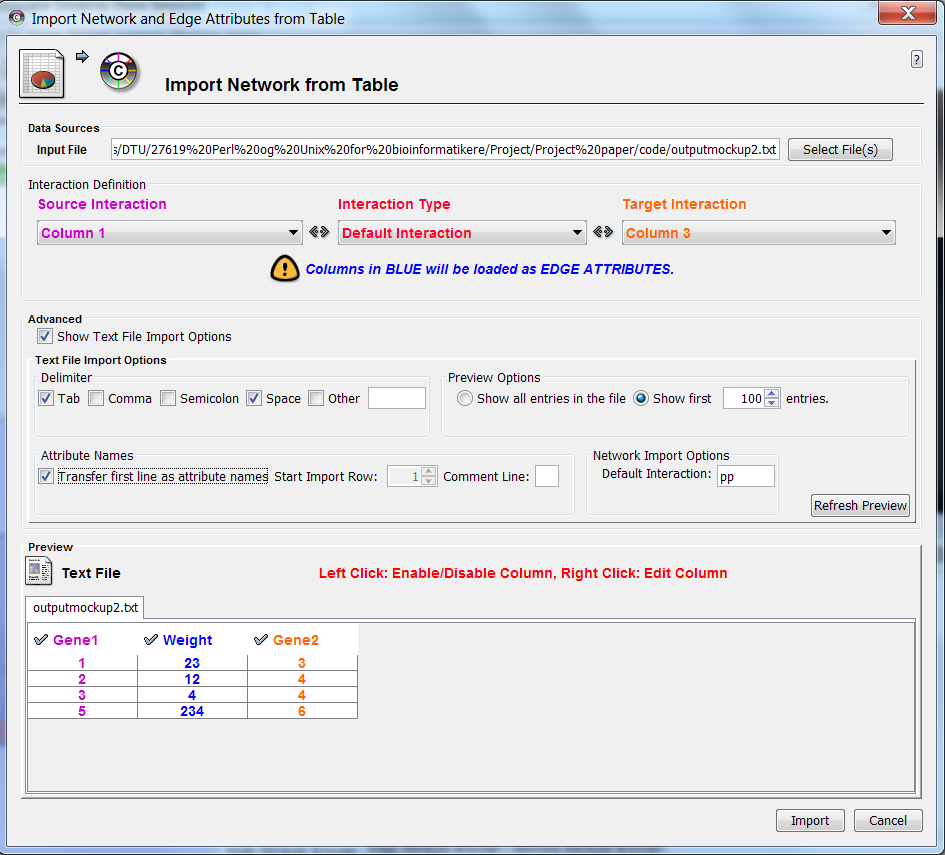
\includegraphics[scale=0.60]{./pictures/cytoscape-options.png}

Then I clicked 'Import' and rendered the network. In order to see the weighted network I choose Layout/Cytoscape Layout/Edge-Weighted Force-Directed (Biolayout)/weighted. Below is a picture of the mock-up network\\

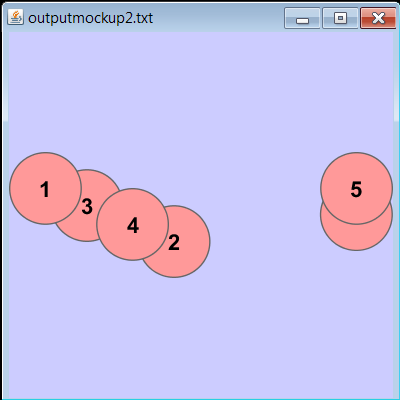
\includegraphics[scale=0.70]{./pictures/cytoscape-network.png}\\


The larger the weight is, the more the edges of the notes overlap.

\newpage

%\section*{Project description}

\subsection*{Description}
Mine NCBI databases for networks of human genes which are connected by the fact that they have been mentioned in the same PubMed article. This project is a good example of how research can be done in Real Life and contains a high degree of freedom in how you want to proceed. Part of the problem is to understand and subsequently parse the NCBI databases, which are flat files. The information found could use used for pathway analysis and construction, disease gene finding and many other purposes, where the underlying problem is to find connections between (novel) genes.

\subsection*{Input and output}
The databases can be found at ftp://ftp.ncbi.nih.gov/gene/DATA/. They can be given to the program in any way you think is sensible. You can also preprocess the databases if you wish. The files of interest are gene2pubmed.gz, gene\_info.gz and README. README simply describes the files in the directory.
The output should be the important networks of genes, displayed in such a way that it is clear, why the network is important, which genes are part of the network and how strongly they are connected. It should be possible to generate a network representation via a third-hand tool from (parts of) the output. The third-hand tool could be Cytoscape.

\subsection*{Details}
In this project we are only interested in human genes. The taxonomy ID (tax\_id) is 9606 for Homo Sapiens and you can use that directly in the program, IF you can explain how you found the number.
The information that the program is supposed to create/mine can be considered to be a graph, where the nodes are genes, and the edges between nodes are links between the genes. Two genes are linked if they are mentioned/connected to the same article. The weight of the edge is the number of articles, which connects to both genes. The greater the weight of the edge, the more important is the relationship of the genes. The data in gene2pubmed is basically a connection between one gene and one PubMed article on each line. From that information you can generate the graph.
How to determine the importance of the network? There are several yardsticks that springs to mind: 1) Number of nodes (many genes), 2) Sum of the edges (many co-mentioning articles), 3) Edge-sum/Nodes (high importance of the network).
Some nodes in the graph do not have any connecting edges, these are uninteresting. Networks that consists of only few nodes where the connecting edges have low weights, are also uninteresting.

\end{document}